Using Routh-Hurwitz analysis, answer the following questions about the block diagram below (assume $K>0$):
\begin{enumerate}
\item Determine the value of $K$ that will make this system unstable (If there is one).
\item If this system does go unstable for this value of $K$, how many unstable poles are there?
\item Is there a value of $K$ greater than the value found in part (a) in which the system becomes stable again?
\end{enumerate}

\begin{center}
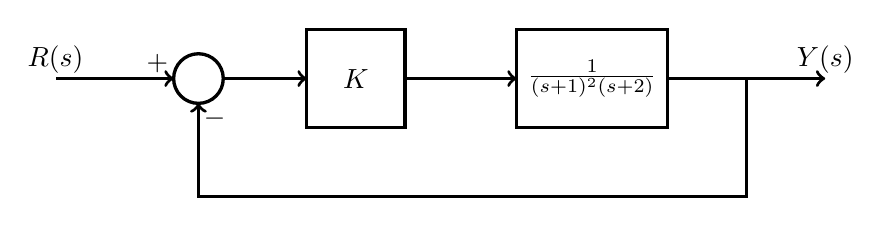
\begin{tikzpicture}[scale=1,inner sep=0pt,outer sep=0pt,very thick,
sysblock/.style={draw,rectangle,inner sep=4pt,minimum width=1.25cm,minimum height=1.25cm,very thick}]

\draw (-2,0) node[draw,circle] (sum1) {$\rule{0pt}{18pt}$};
\draw (0,0) node[sysblock] (K)  {$K$};
\draw (3,0) node[sysblock] (G) {$\frac{1}{(s+1)^2(s+2)}$};
\draw[<-] (sum1.180) node[above left=2pt] {$+$} -- ++(-1.5,0) node[above=2pt] {$R(s)$};
\draw[->] (sum1.0) -- (K.180);
\draw[->] (K.0) -- (G.180);
\draw[->] (G.0) --  ++(2,0) node[above=2pt] {$Y(s)$};
\draw[->] (G.0) -- ++(1,0) -- ++(0,-1.5) -| (sum1.-90) node[below right=2pt] {$-$};
\end{tikzpicture}
\end{center}
